\clearpage
\section{Chapter five}

% %%%%%%%%%%%%%%%%%%%%%%%%%%%%%%%%%%%%%%%%%%%%%%%%%%%%%%%
%
% %%%%%%%%%%%%%         SECTION           %%%%%%%%%%%%%%
%
% %%%%%%%%%%%%%%%%%%%%%%%%%%%%%%%%%%%%%%%%%%%%%%%%%%%%%%%


\vspace*{\fill}

\begin{example}
  \centering
  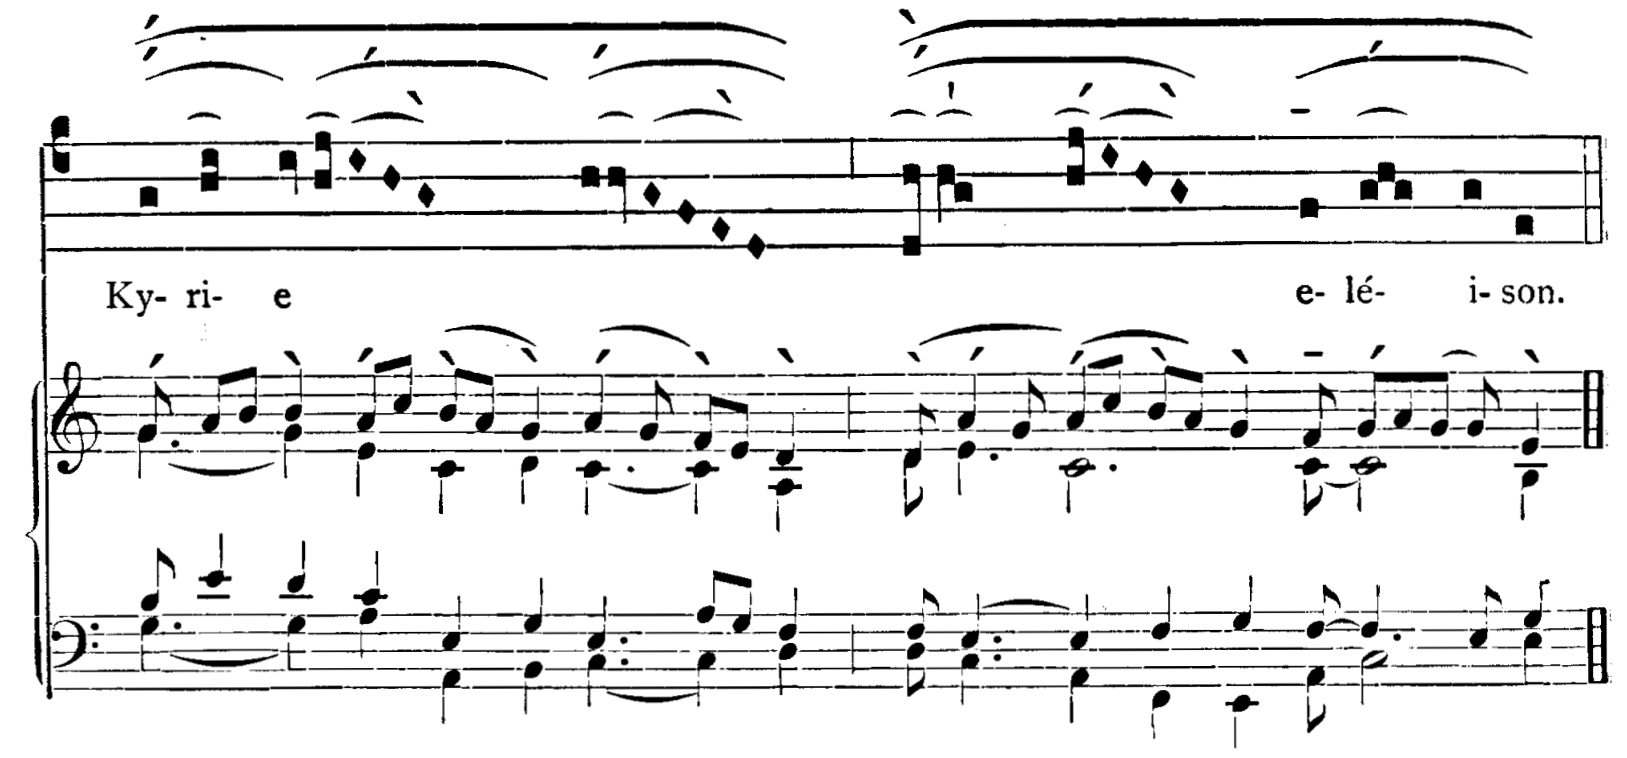
\includegraphics[width=\linewidth]{c/4/ex/springer_221.png}
  \caption{Springer, Accompaniment based on rhythmic analysis, 1908}
  \label{mus:springer_221}
\end{example}

\vspace*{\fill}

\begin{landscape}

  \vspace*{\fill}

  \begin{example}
    \centering
    \includegraphics[width=\linewidth]{c/5/ex/springer_halfdim_16.png}
    \caption{Springer, Use of half-diminished chord, 1910}
    \label{mus:springer_halfdim_16}
  \end{example}

  \vspace*{\fill}

\end{landscape}

  \vspace*{\fill}

  \begin{example}
    \centering
    \includegraphics[width=\linewidth]{c/4/ex/renner_deo_5.png}
    \caption{Renner, Chromatic accompanying parts, 1914}
    \label{mus:renner_deo_5}
  \end{example}

\vspace*{\fill}

\newpage

\vspace*{\fill}

\begin{example}
  \centering
  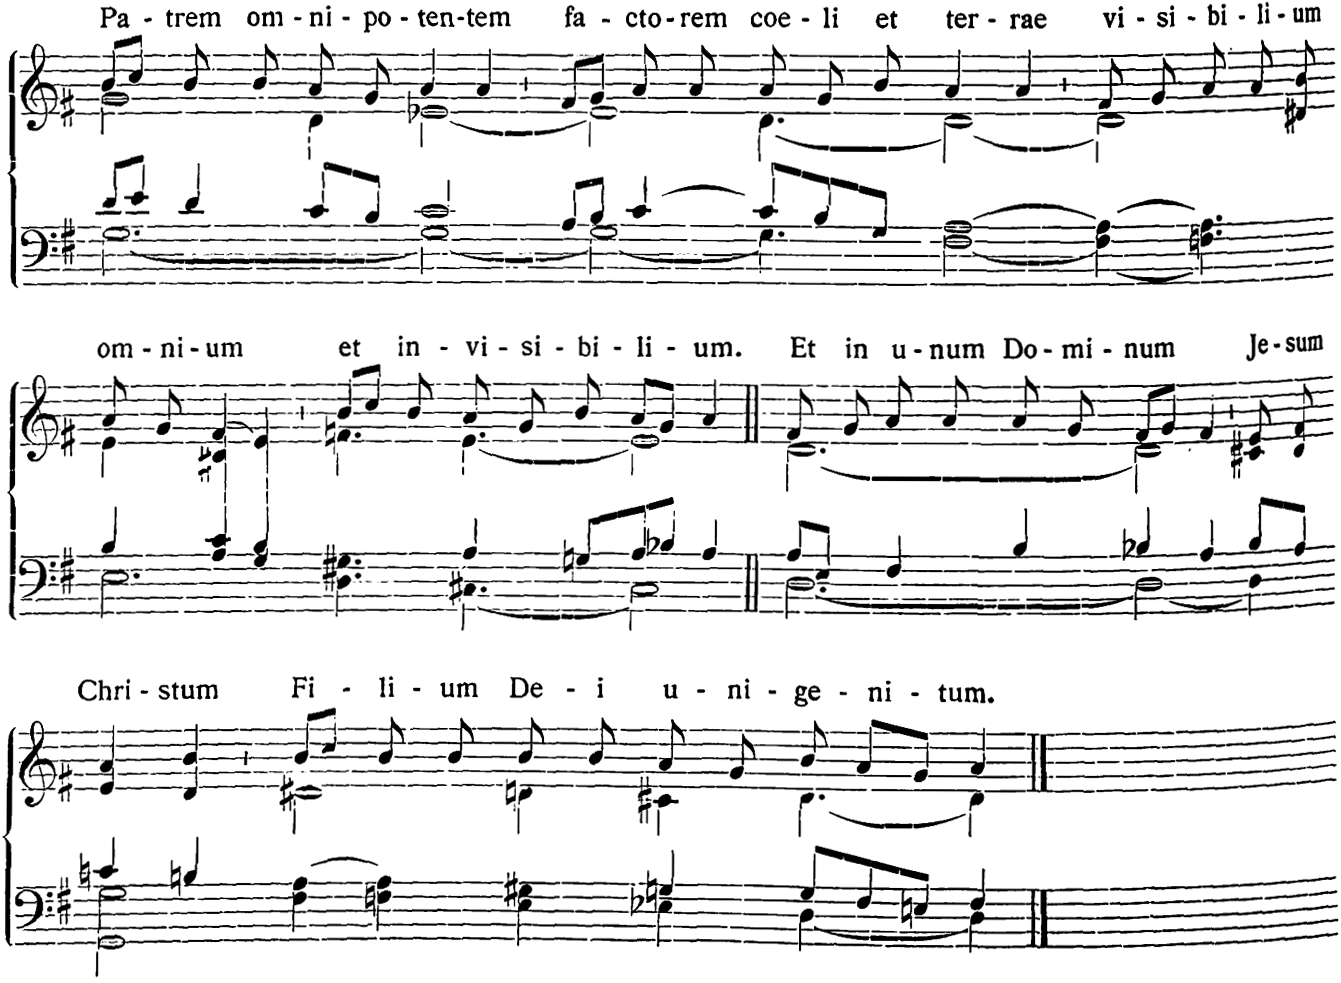
\includegraphics[width=\linewidth]{c/5/ex/griesbacher_credo_202.png}
  \caption{Griesbacher, Chromatic \emph{Credo} accompaniment, 1912}
  \label{mus:griesbacher_credo_202}
\end{example}

\vspace*{\fill}

\newpage

\vspace*{\fill}

\begin{example}
  \centering
  \includegraphics[width=.9\linewidth]{c/5/ex/griesbacher_ideal_88.png}
  \caption{Griesbacher's ideal method of accompaniment, 1912}
  \label{mus:griesbacher_ideal_88}
\end{example}

\vspace*{\fill}

\newpage

\vspace*{\fill}

\begin{example}
  \centering
  \includegraphics[width=\linewidth]{c/5/ex/molitor_melisma_99.jpg}
  \caption{Molitor, `Concertant'-type accompaniment, 1913}
  \label{mus:molitor_melisma_99}
\end{example}

\vspace*{\fill}

\newpage

\vspace*{\fill}

\begin{example}
  \centering
  \includegraphics[width=\linewidth]{c/4/ex/ranse.jpg}
  \caption{De Ranse, `Concertant'-type accompaniment, \emph{c}.1909}
  \label{mus:deranse_ascension}
\end{example}

\vspace*{\fill}

\newpage

  \vspace*{\fill}

  \begin{example}
    \centering
    \includegraphics[width=\linewidth]{c/4/ex/wismeyer_sustained.png}
    \caption{Wismeyer, Accompaniment above pitch of chant, 1933}

    \label{mus:wismeyer_sustained}
  \end{example}

  \vspace*{\fill}

  \begin{example}
    \centering
    \includegraphics[width=\linewidth]{c/4/ex/peeters_angelis_73.png}
    \caption{Peeters, \emph{Ibid}., 1949}
    \label{mus:peeters_angelis_73}
  \end{example}

  \vspace*{\fill}

\newpage

\vspace*{\fill}

\begin{example}
  \centering
  \includegraphics[width=\linewidth]{c/4/ex/emmanuel_traite_102.jpg}
  \caption{Emmanuel, Accompaniment for children's voices, 1913}
  \label{mus:emmanuel_traite_102}
\end{example}

\vspace*{\fill}

\newpage

\vspace*{\fill}

\begin{example}
  \centering
  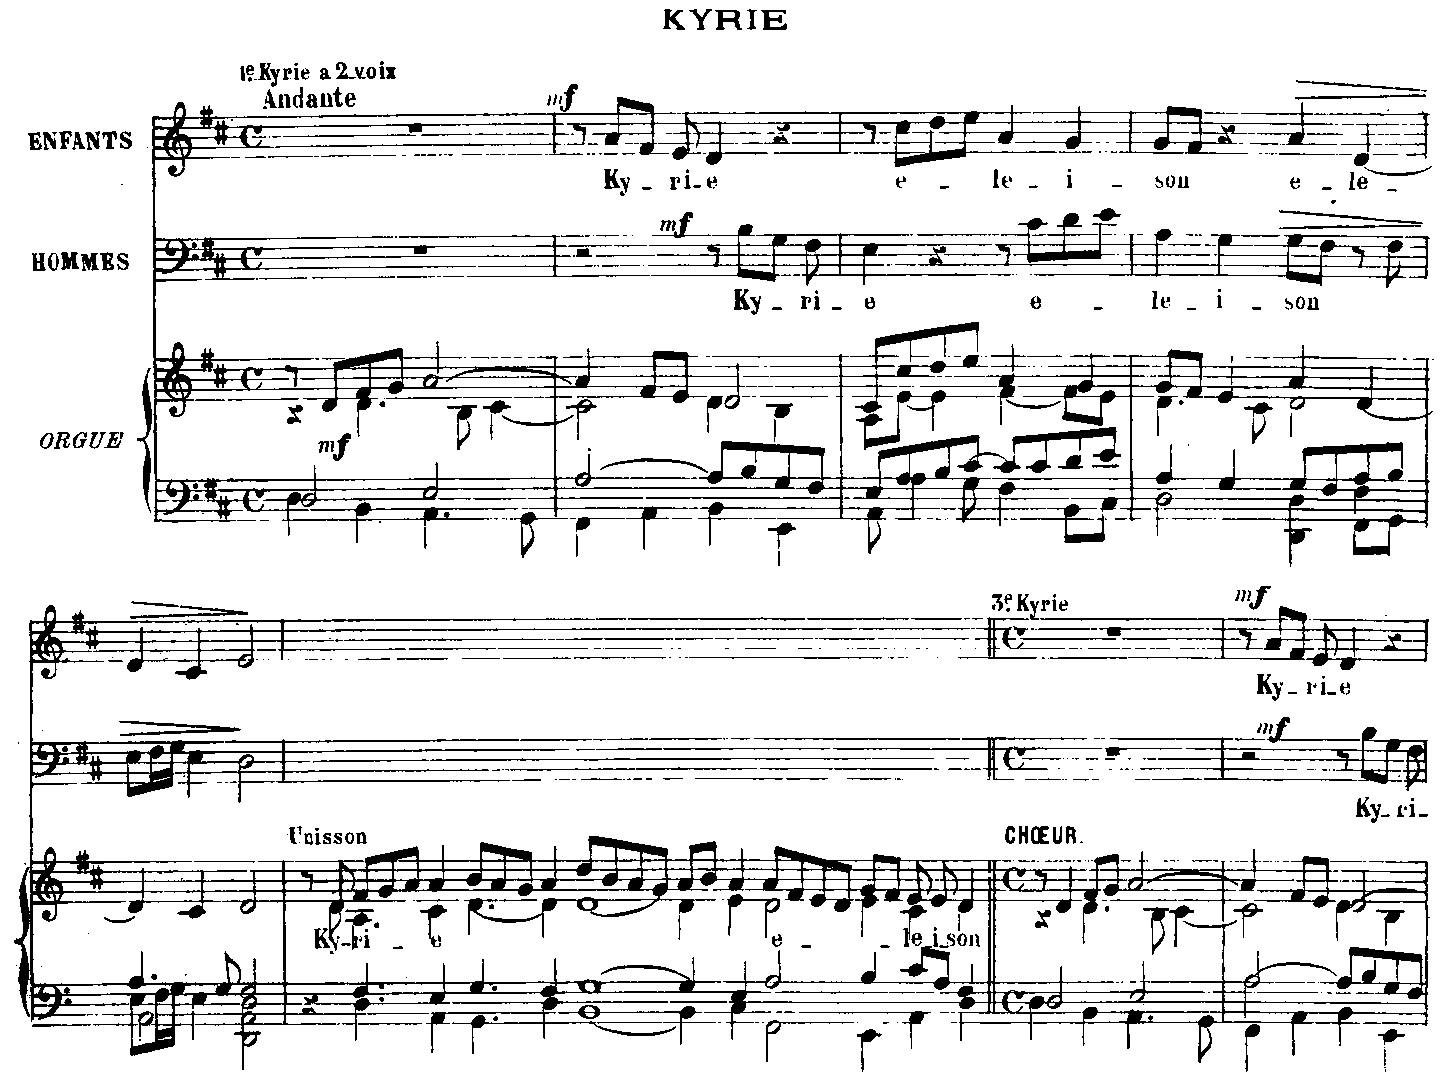
\includegraphics[width=\linewidth]{c/4/ex/perruchot_interlineal.png}
  \caption{Perruchot, Interlineal accompaniment, 1910}
  \label{mus:perruchot_interlineal}
\end{example}

\vspace*{\fill}

\newpage

\vspace*{\fill}

\begin{example}
  \centering
  \includegraphics[width=.9\linewidth]{c/5/ex/bas_antcons_116.png}
  \caption{Bas, Indicating `protase' and `apodose', 1911}
  \label{mus:bas_antcons_116}
\end{example}

\vspace*{\fill}

\begin{example}
  \centering
  \includegraphics[width=\linewidth]{c/5/ex/bas_kyriesustained_149.png}
  \caption{Bas, More sustained accompaniment, 1911}
  \label{mus:bas_kyriesustained_149}
\end{example}

\vspace*{\fill}

\newpage

\vspace*{\fill}

\begin{example}
  \centering
  \includegraphics[width=\linewidth]{c/4/ex/bas_compose.jpeg}
  \caption{Bas, Accompaniment segues into postlude, \emph{c}.1915}
  \label{mus:bas_compose}
\end{example}

\vspace*{\fill}

\newpage

\vspace*{\fill}

\begin{example}
  \centering
  \includegraphics[width=\linewidth]{c/4/ex/zerr_ordo_2.jpg}
  \caption{Zerr, Additive conjunct motion, 1937}
  \label{mus:zerr_ordo_2}
\end{example}


\vspace*{\fill}

\begin{example}
  \centering
  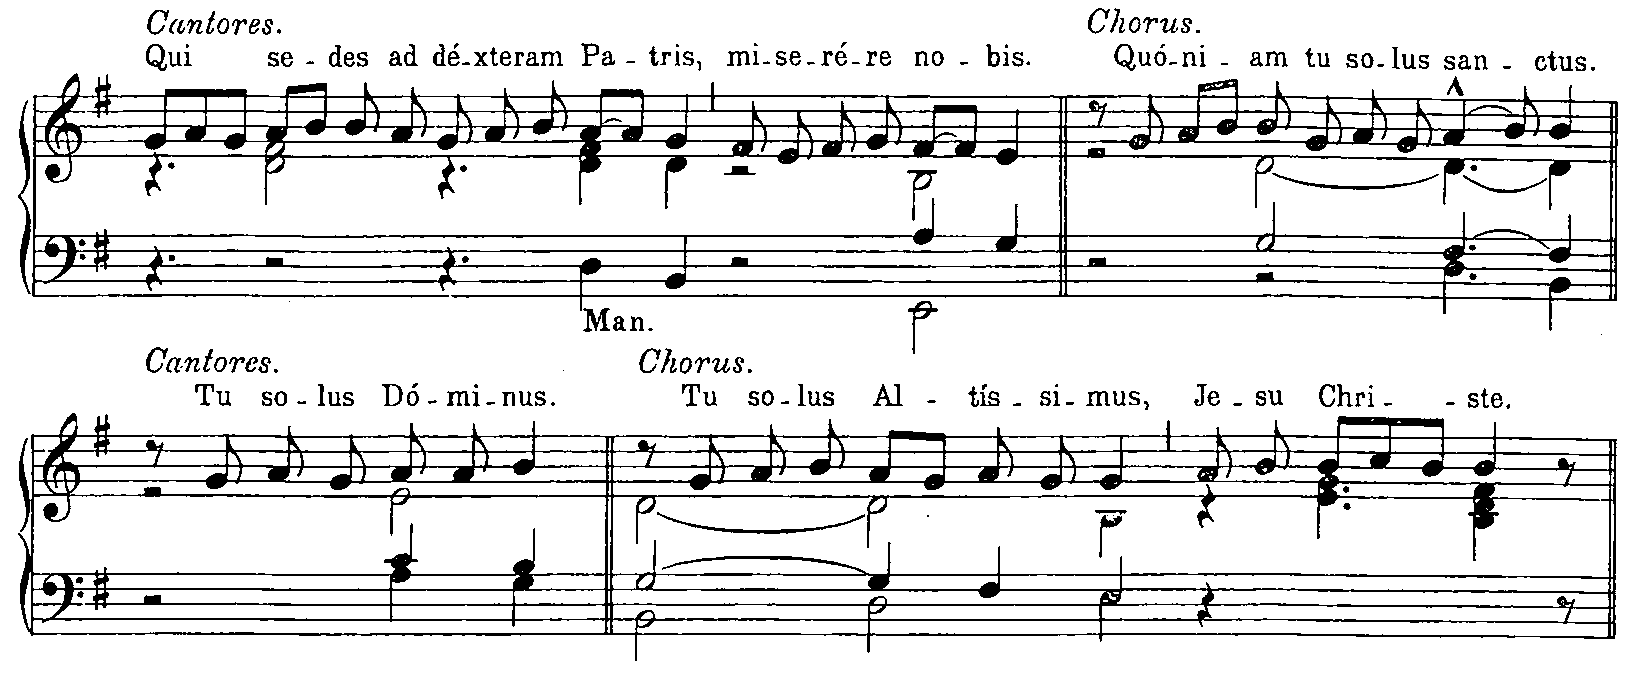
\includegraphics[width=\linewidth]{c/4/ex/bas_qui_33.png}
  \caption{Bas, Higher quantity of parts at cadences, 1921}
  \label{mus:bas_qui_33}
\end{example}

\vspace*{\fill}

\newpage

\vspace*{\fill}

\begin{example}
  \centering
  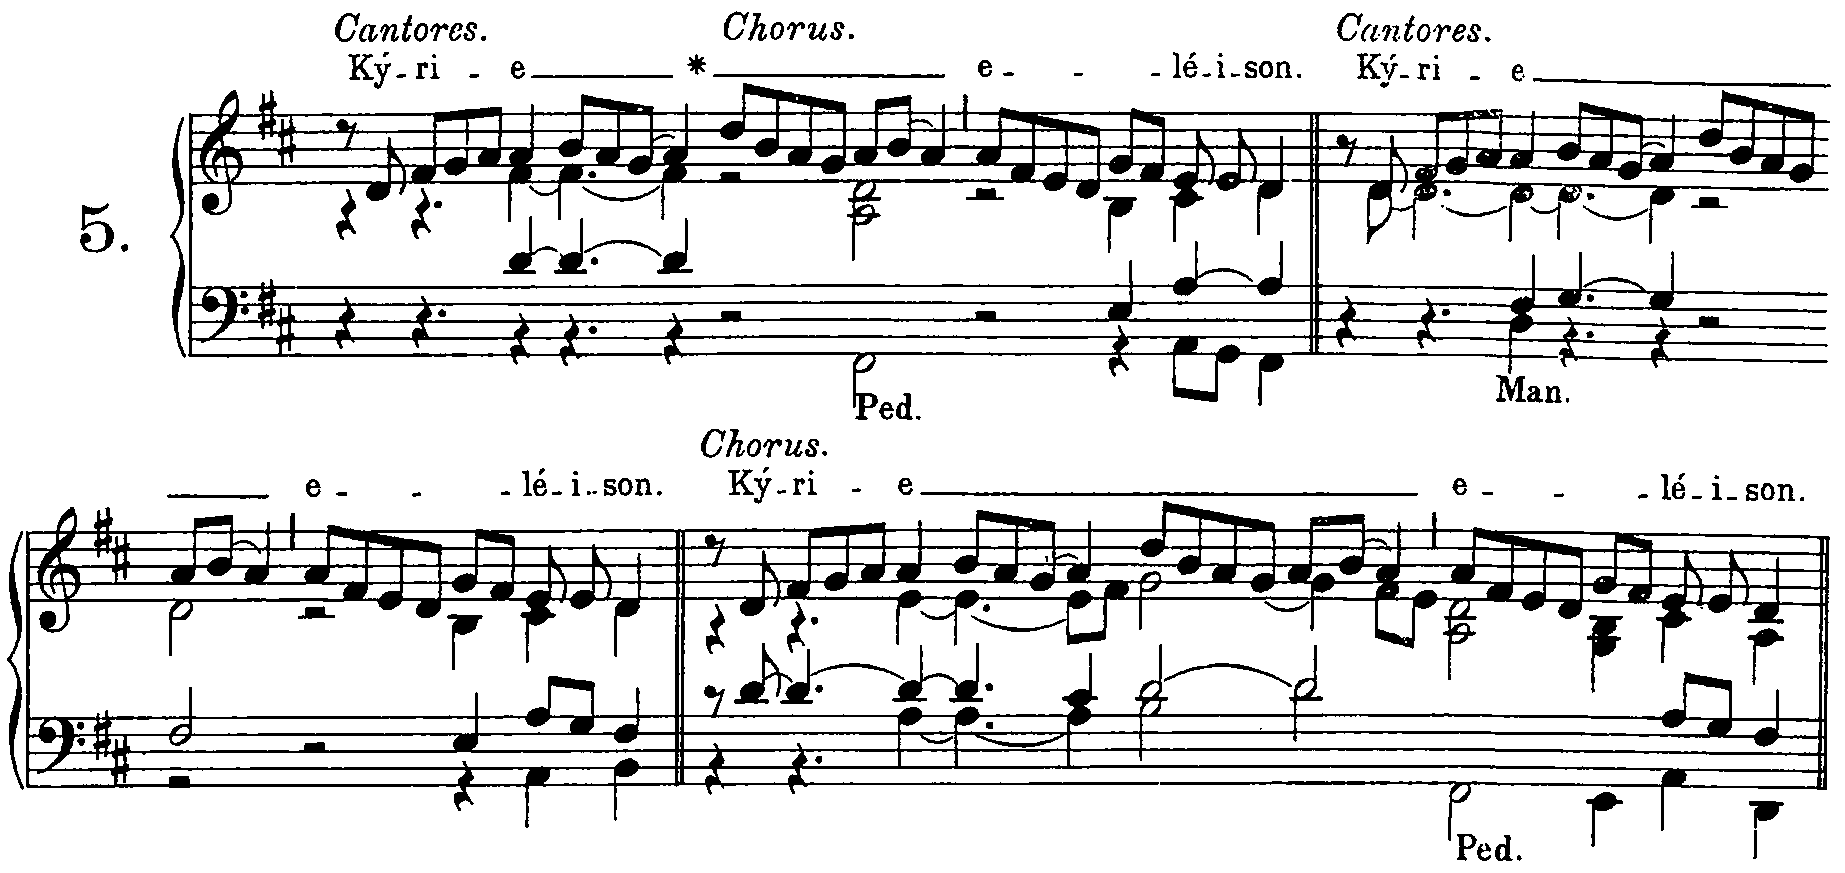
\includegraphics[width=\linewidth]{c/4/ex/bas_angelis_35.png}
  \caption{Bas, Suspension persists through rest, 1921}
  \label{mus:bas_angelis_35}
\end{example}

\vspace*{\fill}

\begin{example}
  \centering
  \includegraphics[width=\linewidth]{c/4/ex/bas_ethomo_78.png}
  \caption{Bas, Delayed resoluation of dissonance, 1921}
  \label{mus:bas_ethomo}
\end{example}

\vspace*{\fill}

\newpage

\vspace*{\fill}

\begin{example}
  \centering
  \includegraphics[width=\linewidth]{c/4/ex/bas_sustainedstyle_kyriale.png}
  \caption{Bas, Agnus VIII as published, 1921}
  \label{mus:bas_sustained_kyriale}
\end{example}

\vspace*{\fill}

\begin{example}
  \centering
  \includegraphics[width=\linewidth]{c/4/ex/bas_sustained_traite1.png}
%  \includegraphics[width=.5\linewidth]{c/4/ex/bas_sustained_traite2.png}
  \caption{Bas, Agnus VIII accompanied in the desired style, 1923}
  \label{mus:bas_sustained_traite}
\end{example}

\vspace*{\fill}

% %%%%%%%%%%%%%%%%%%%%%%%%%%%%%%%%%%%%%%%%%%%%%%%%%%%%%%%
%
% %%%%%%%%%%%%%         SECTION           %%%%%%%%%%%%%%
%
% %%%%%%%%%%%%%%%%%%%%%%%%%%%%%%%%%%%%%%%%%%%%%%%%%%%%%%%


\begin{landscape}

  \vspace*{\fill}

  \begin{example}
    \centering
    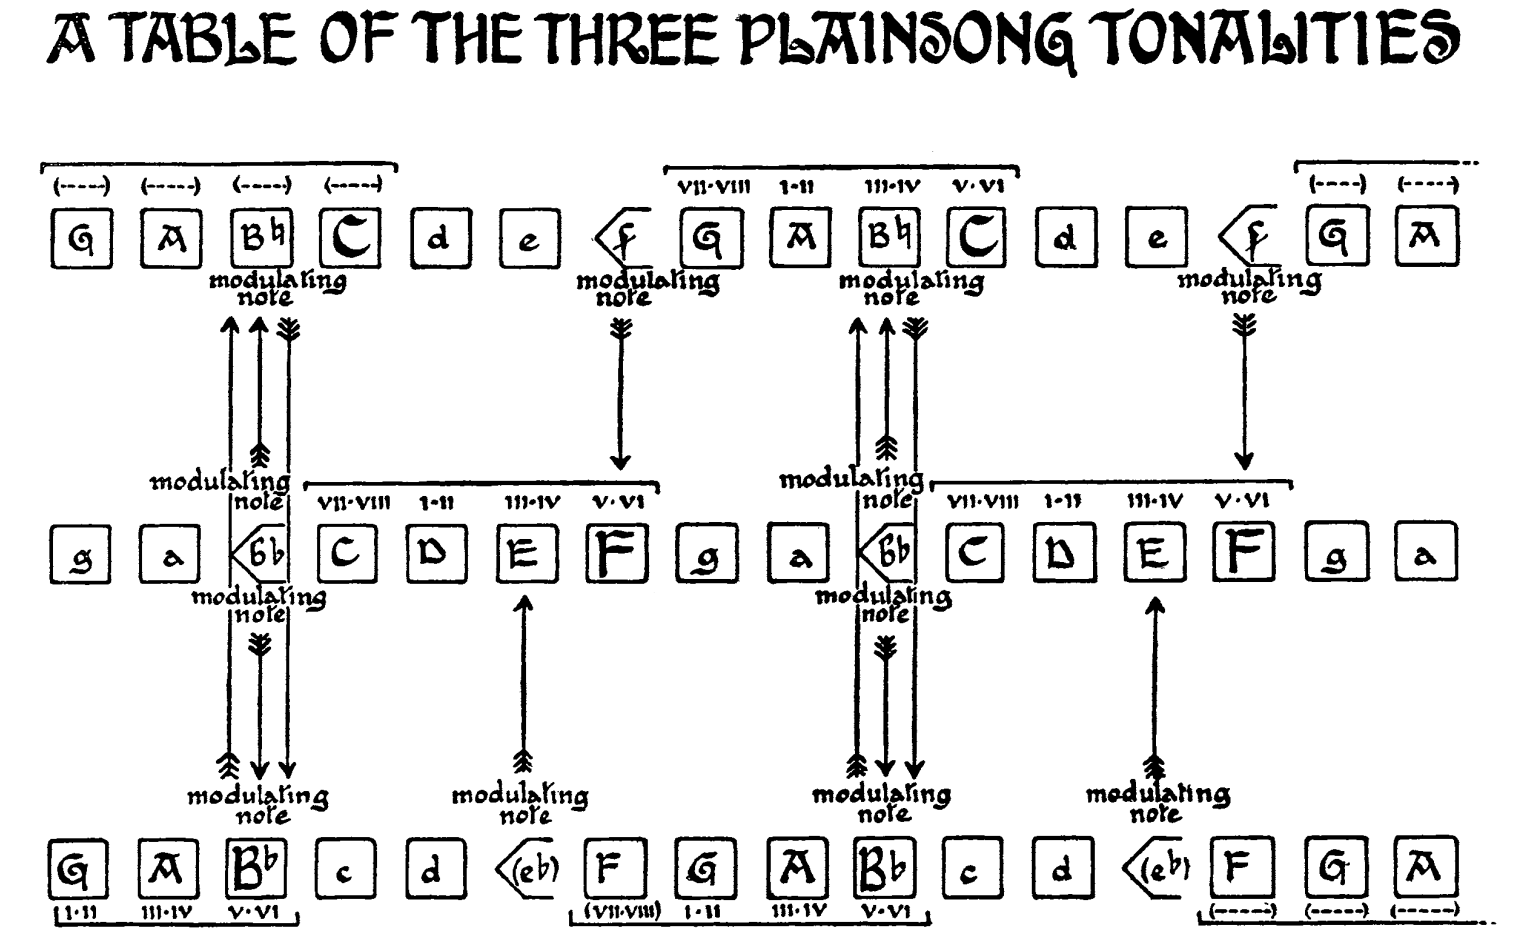
\includegraphics[width=.7\linewidth]{c/4/ex/three_tonalities.png}
    \caption{Desrocquettes-Potiron, Three plainsong tonalities, 1924, 1927, 1933}
    \label{mus:three_tonalities}
  \end{example}

  \vspace*{\fill}

\end{landscape}

\vspace*{\fill}

\begin{example}
  \centering
  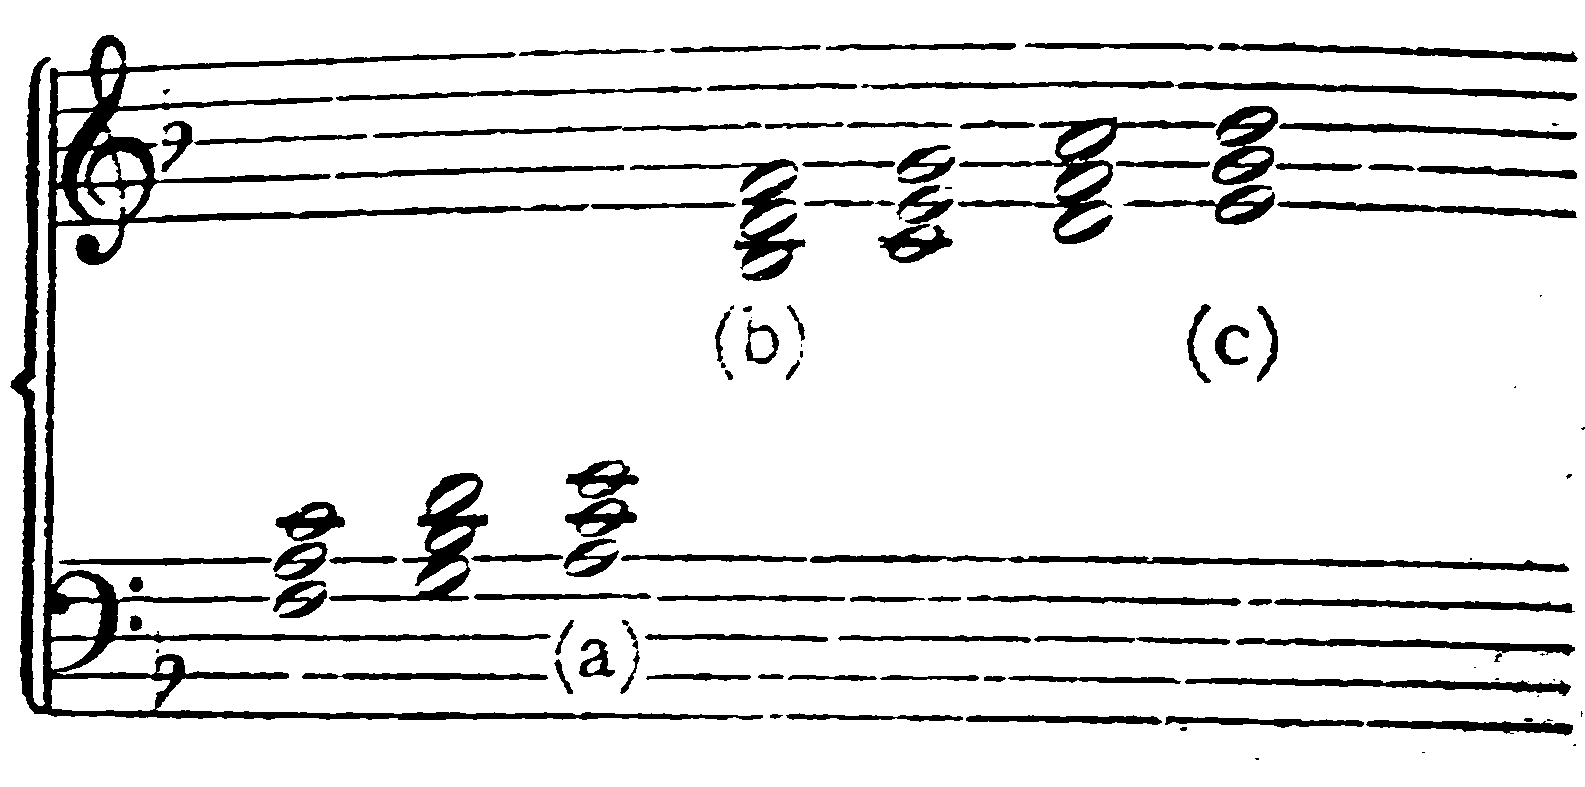
\includegraphics[width=.7\linewidth]{c/4/ex/dd_fscale.png}
  \caption{Desrocquettes, Proposing chords for \emph{Fa} \emph{tonalité}, 1924}
  \label{mus:dd_fscale}
\end{example}

\vspace*{\fill}

\begin{example}
  \centering
  \includegraphics[width=.7\linewidth]{c/4/ex/dd_cscale.png}
  \caption{Desrocquettes, Those for the \emph{Do}, 1924}
  \label{mus:dd_cscale}
\end{example}

\vspace*{\fill}

\begin{example}
  \centering
  \includegraphics[width=.7\linewidth]{c/4/ex/dd_bflatscale.png}
  \caption{Desrocquettes, Those for the \emph{Si}\kern 1pt\flat{} \emph{tonalité}, 1924}
  \label{mus:dd_bflatscale}
\end{example}

\vspace*{\fill}

\newpage

\vspace*{\fill}

\begin{example}
  \centering
  \includegraphics[width=.9\linewidth]{c/4/ex/potirondesrocquettes_29pieces.jpg}
  \caption{Desrocquettes, Adding of groups in pencil, 1929}
  \label{mus:potirondesrocquettes_29pieces}
\end{example}

\vspace*{\fill}

\newpage

\vspace*{\fill}


\begin{example}
  \centering
  \includegraphics[width=\linewidth]{c/4/ex/potiron_parse.png}
  \caption{Potiron, Ascensiontide Alleluia parsed into modal groups, 1927/1933}
  \label{mus:potiron_parse}
\end{example}

\vspace*{\fill}

\begin{example}
  \centering
  \includegraphics[width=\linewidth]{c/4/ex/examen1925.jpg}
  \caption{Anonymous example from final exam at the Institut grégorien, 1925}
  \label{mus:examen1925}
\end{example}

\vspace*{\fill}

\newpage

\vspace*{\fill}

\begin{example}
  \centering
  \includegraphics[width=.85\linewidth]{c/4/ex/desrocquettes_agnus.png}
  \caption{Desrocquettes, Harmonising group II with pitches in group I, 1925}
  \label{mus:desrocquettes_agnus}
\end{example}

\vspace*{\fill}

\newpage

\vspace*{\fill}


\begin{example}
  \centering
  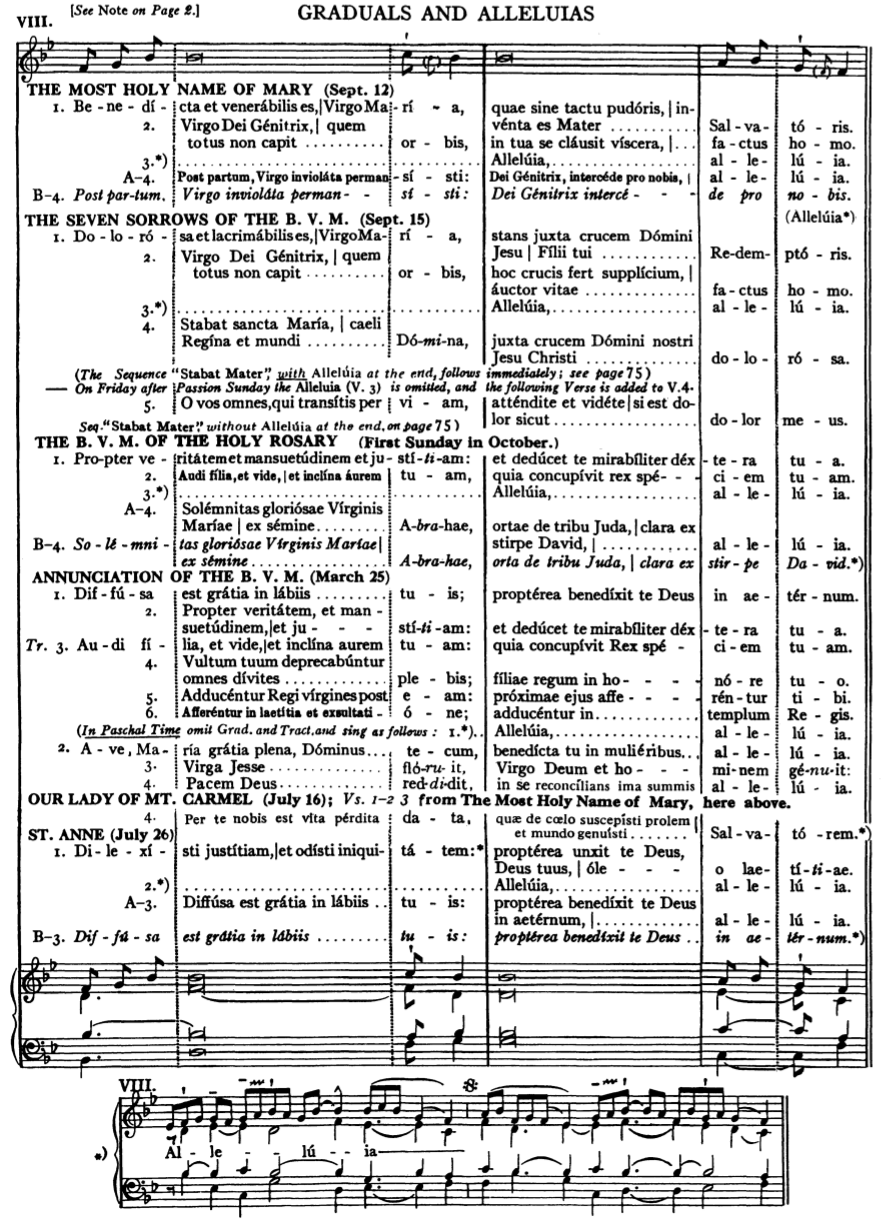
\includegraphics[width=.8\linewidth]{c/4/ex/rossini_proper_56.png}
  \caption{Rossini, Proper set to tone and accompaniment, 1957}
  \label{mus:rossini_proper_56}
\end{example}

\vspace*{\fill}

\newpage

%%%%%%%%%%%%%%%%%%%%%%%%%%%%%%%%%%%%%%%%%%%%%%%%%%%%%%%%%%%%%
%                                                           %
%                   Section 5.3                             %
%                                                           %
%%%%%%%%%%%%%%%%%%%%%%%%%%%%%%%%%%%%%%%%%%%%%%%%%%%%%%%%%%%%%

\vspace*{\fill}

\begin{example}
  \centering
  \includegraphics[width=\linewidth]{c/4/ex/holst_sop.png}
  \caption{Holst, Quasi-aleatoric orchestral accompaniment, \emph{c}.1917}
  \label{mus:holst_sop}
\end{example}

\vspace*{\fill}

\newpage

\vspace*{\fill}

\begin{example}
  \centering
  \includegraphics[width=\linewidth]{c/4/ex/holst_ten.png}
  \caption{Holst, Use of 7/5/4/2 chord, \emph{c}.1917}
  \label{mus:holst_ten}
\end{example}

\vspace*{\fill}

\begin{example}
  \centering
  \includegraphics[width=.9\linewidth]{c/6/ex/latry.png}
  \caption{Latry, \emph{Ibid}., 2010}
  \label{mus:latry}
\end{example}

\vspace*{\fill}

\newpage

\vspace*{\fill}

\begin{example}
  \centering
  \includegraphics[width=\linewidth]{c/4/ex/credovi_rev.png}
  \caption{Desrocquettes-Potiron, Credo VI cadence, 1924}
  \label{mus:credovi_revue}
\end{example}

\vspace*{\fill}

\begin{example}
  \centering
  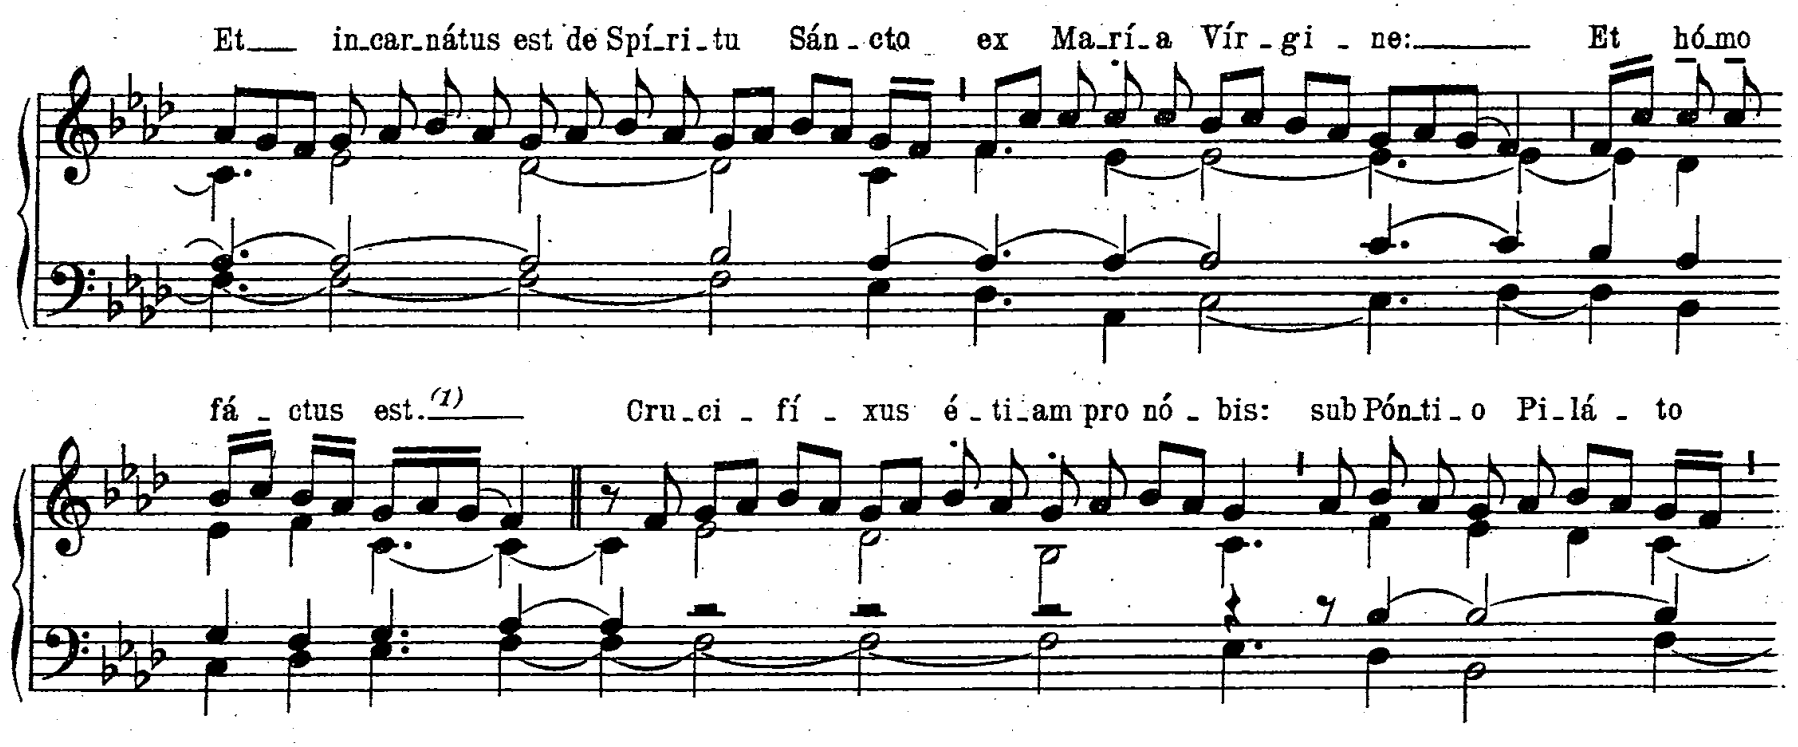
\includegraphics[width=\linewidth]{c/4/ex/credovi_kyriale.png}
  \caption{Desrocquettes-Potiron-Caplet, Revised Credo VI cadence, 1925}
  \label{mus:credovi_kyriale}
\end{example}

\vspace*{\fill}

\begin{landscape}

\vspace*{\fill}


\begin{example}
  \centering
  \includegraphics[width=.9\linewidth]{c/4/ex/lapierre_punctuation.png}
  \caption{Lapierre, Pointing, 1946}
  \label{mus:lapierre_punctuation}
\end{example}

\vspace*{\fill}

\end{landscape}

\begin{landscape}

  \vspace*{\fill}

  \begin{example}
    \centering
    \includegraphics[width=.9\linewidth]{c/4/ex/raczkowski_angelis_41.png}
    \caption{Rączkowski, Following Solesmian transcription, 1954}
    \label{mus:raczkowski_angelis_41}
  \end{example}

  \vspace*{\fill}
\end{landscape}

\vspace*{\fill}

\begin{example}
  \centering
  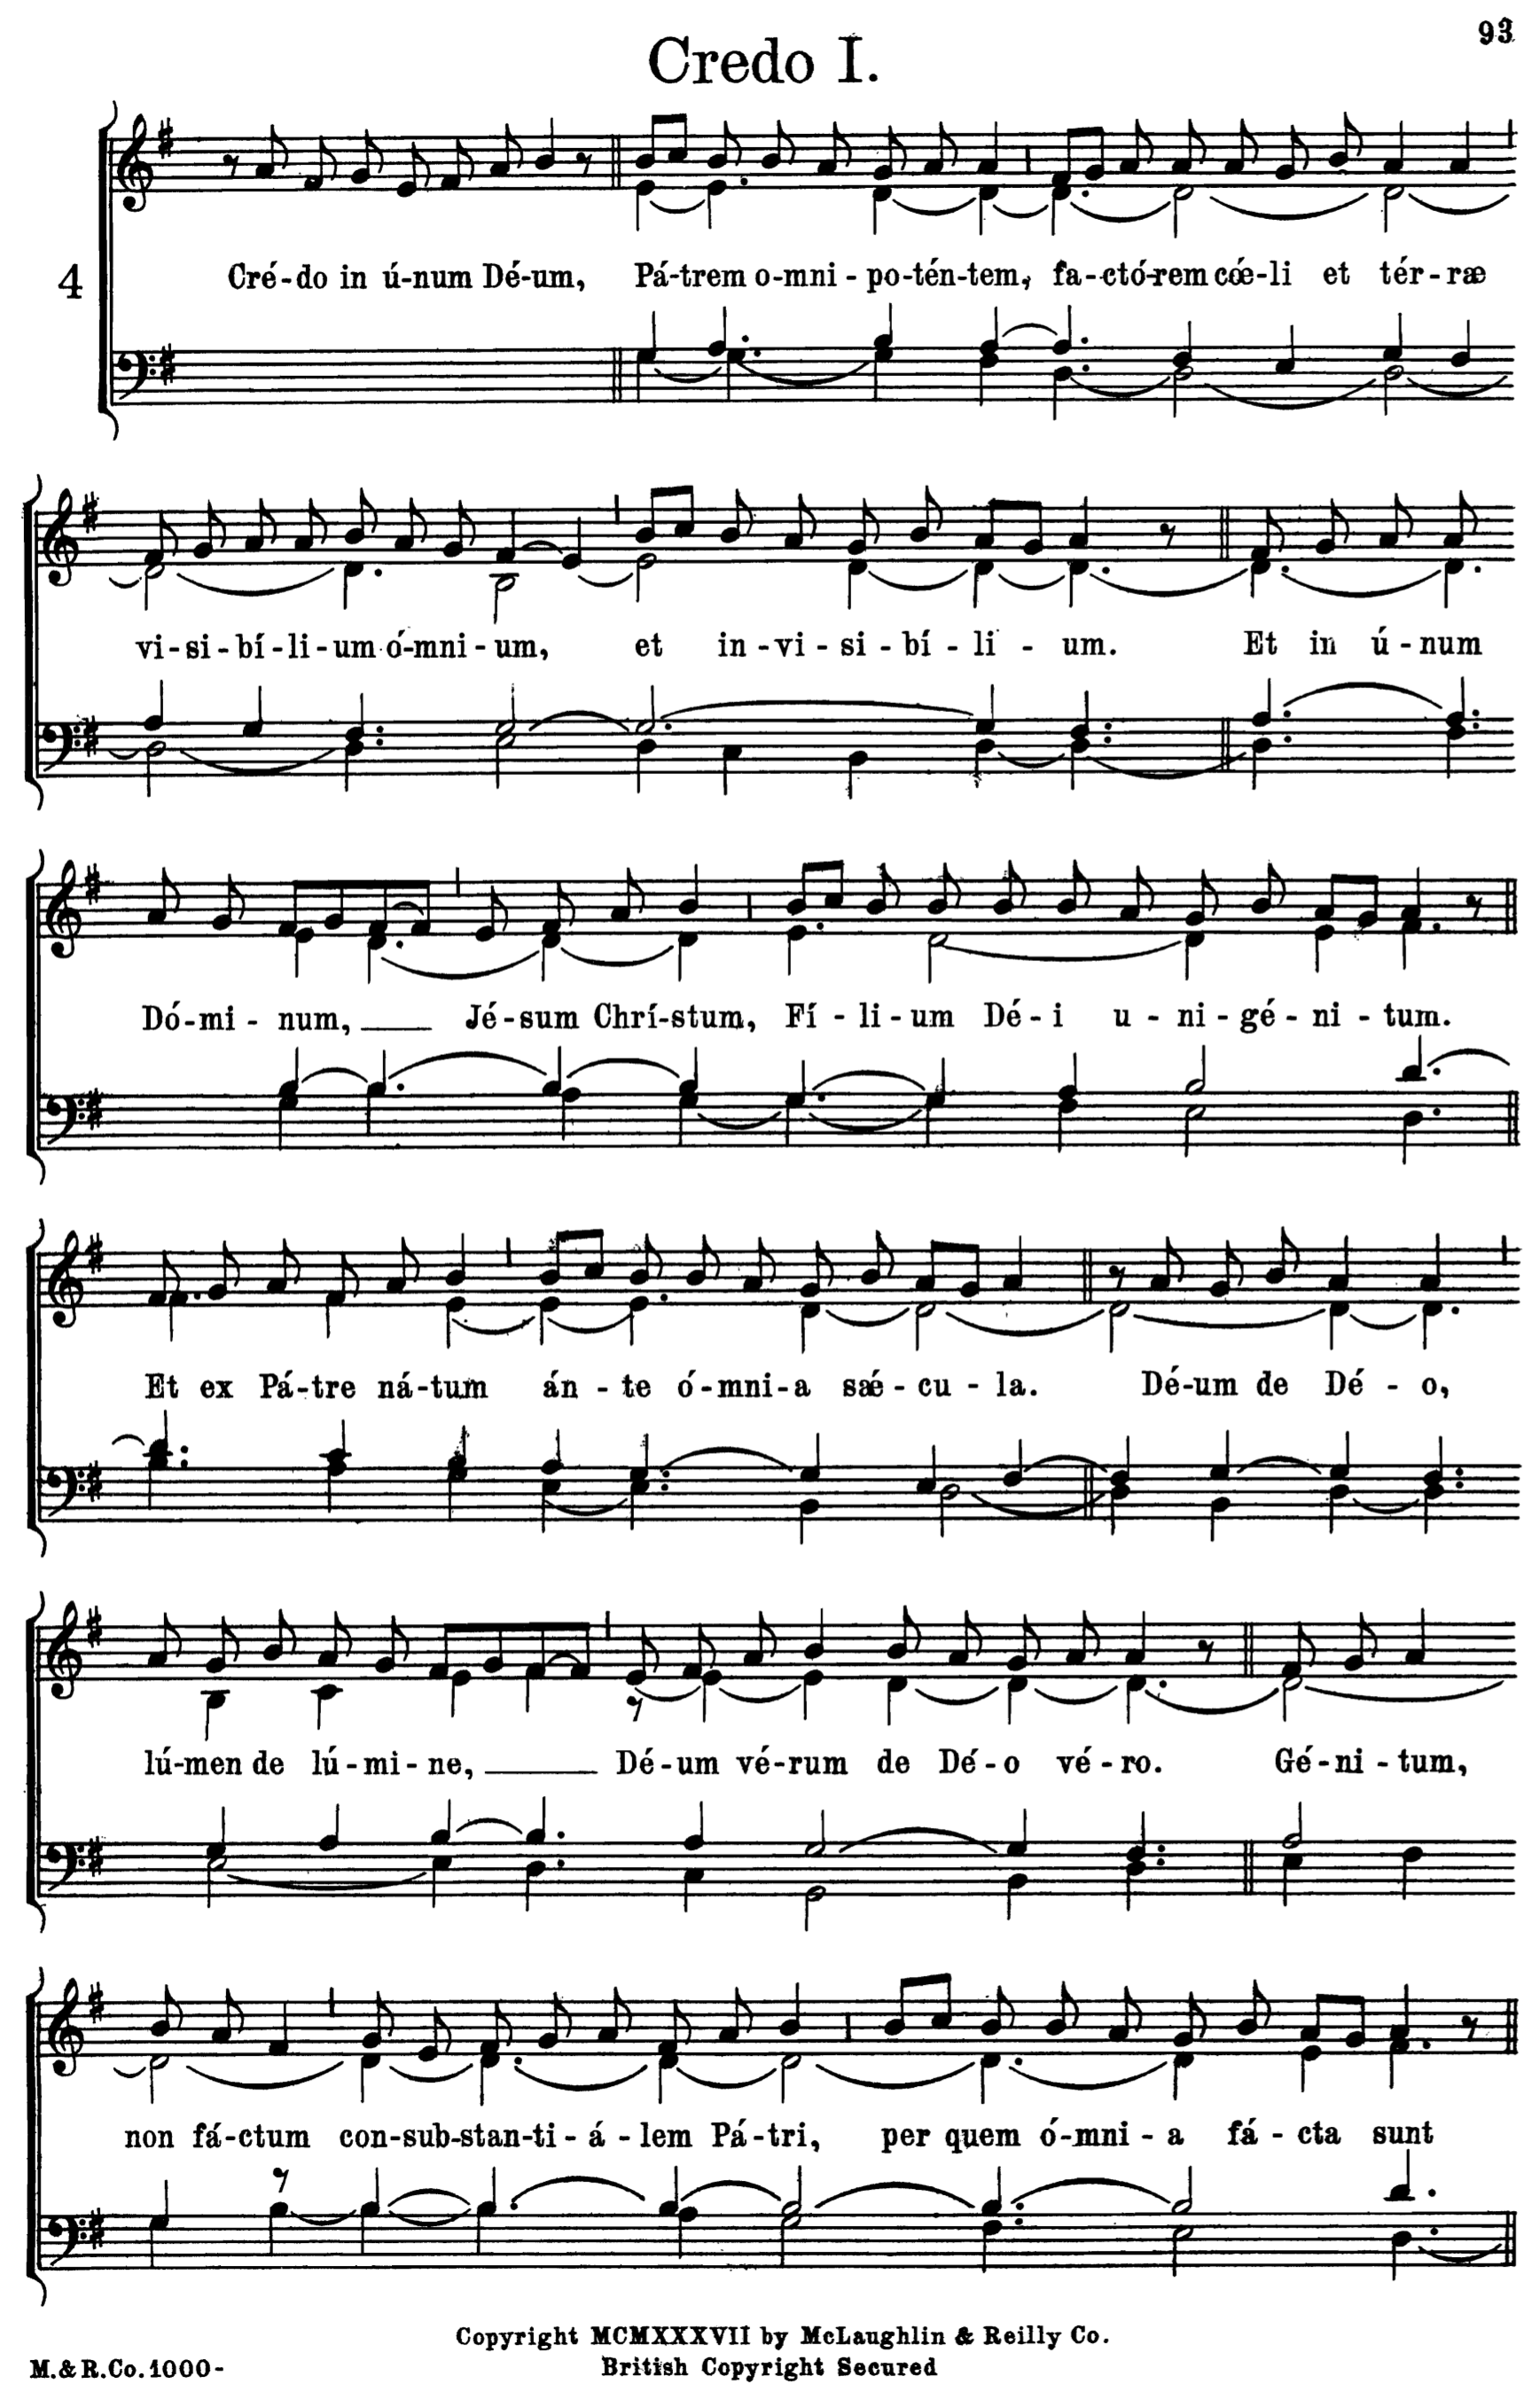
\includegraphics[width=.7\linewidth]{c/4/ex/achille_credo1937_93.png}
  \caption{Bragers, Printed Credo I accompaniment, 1937}
  \label{mus:bragers_credo1}
\end{example}

\vspace*{\fill}

\newpage

\vspace*{\fill}

\begin{example}
  \centering
  \includegraphics[width=\linewidth]{c/5/ex/potiron_circumderunt_60.png}
  \includegraphics[width=\linewidth]{c/5/ex/potiron_circumderunt_61.png}
  \caption{Potiron, Absence of \pitch{4} from the accompaniment, 1933}
  \label{mus:potiron_circumderunt}
\end{example}

\vspace*{\fill}

\begin{example}
  \centering
  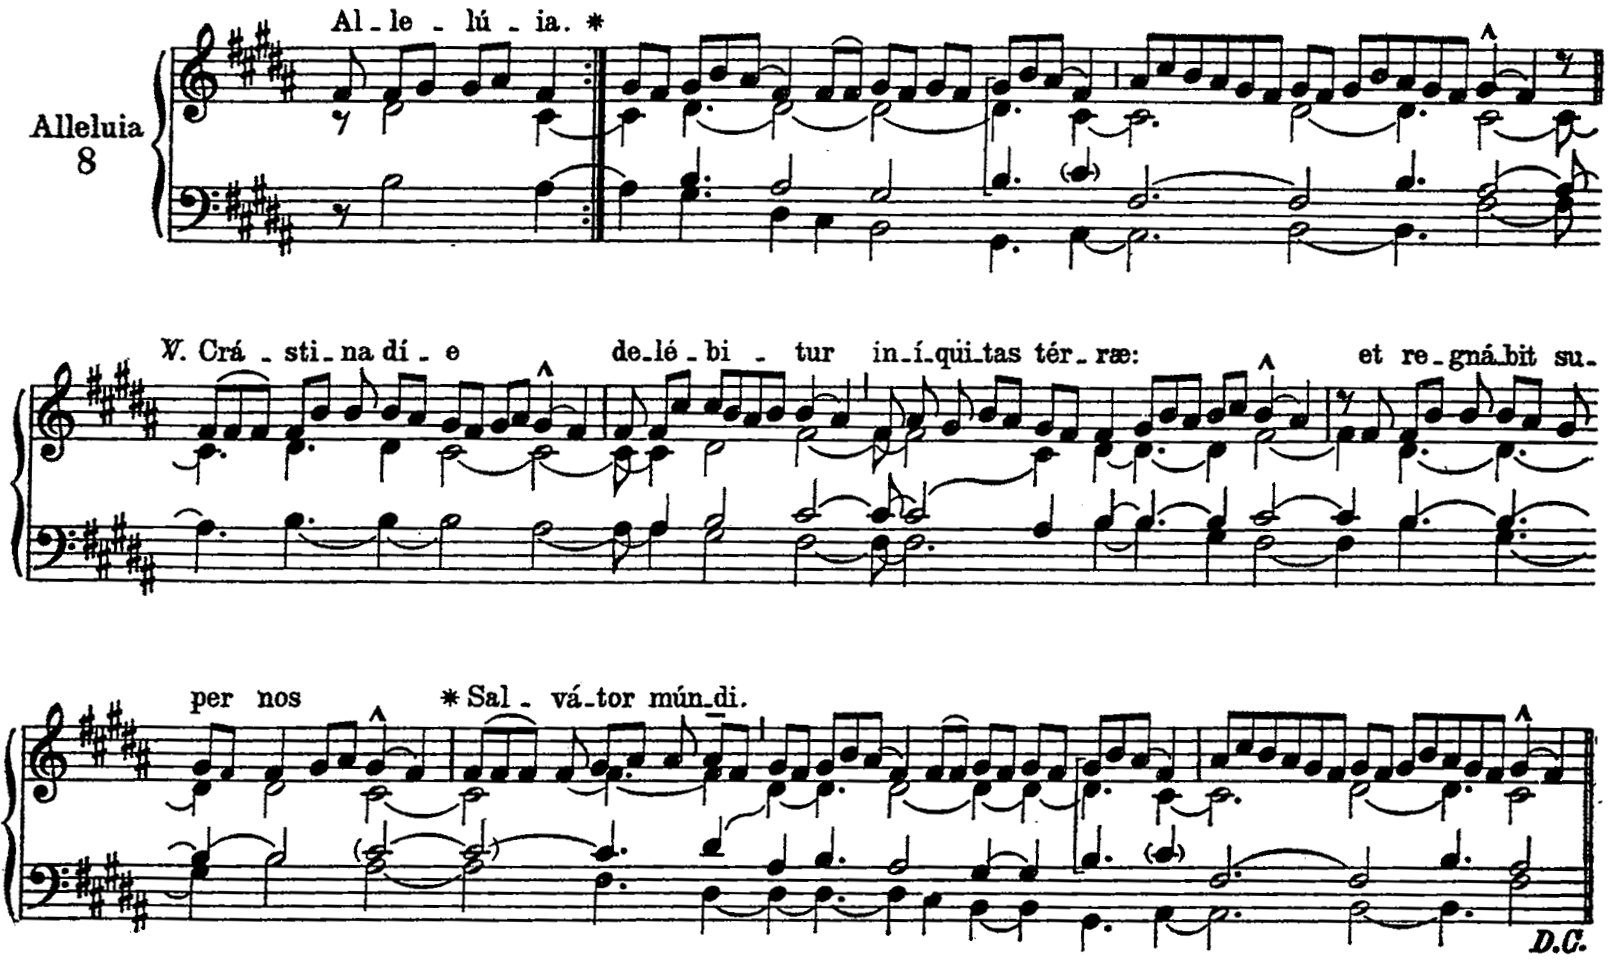
\includegraphics[width=\linewidth]{c/5/ex/potiron_crastina_18.png}
  \caption{Potiron, Avoidance of `E' in the accompaniment, 1933}
  \label{mus:potiron_crastina}
\end{example}

\vspace*{\fill}

\newpage

\vspace*{\fill}

\begin{example}
  \centering
  \includegraphics[width=\linewidth]{c/5/ex/potiron_kyriale_9.JPG}
  \caption{Potiron, Avoidance of `E'\kern 1pt\flat{}, 1950}
  \label{mus:potiron_kyriale_9}
\end{example}

\vspace*{\fill}

\begin{example}
  \centering
  \includegraphics[width=.9\linewidth]{c/5/ex/potiron_deo_9.JPG}
  \caption{Potiron, Use of `E' when not in the chant, 1950}
  \label{mus:potiron_deo_9}
\end{example}

\vspace*{\fill}

\newpage

\vspace*{\fill}

\begin{example}
  \centering
  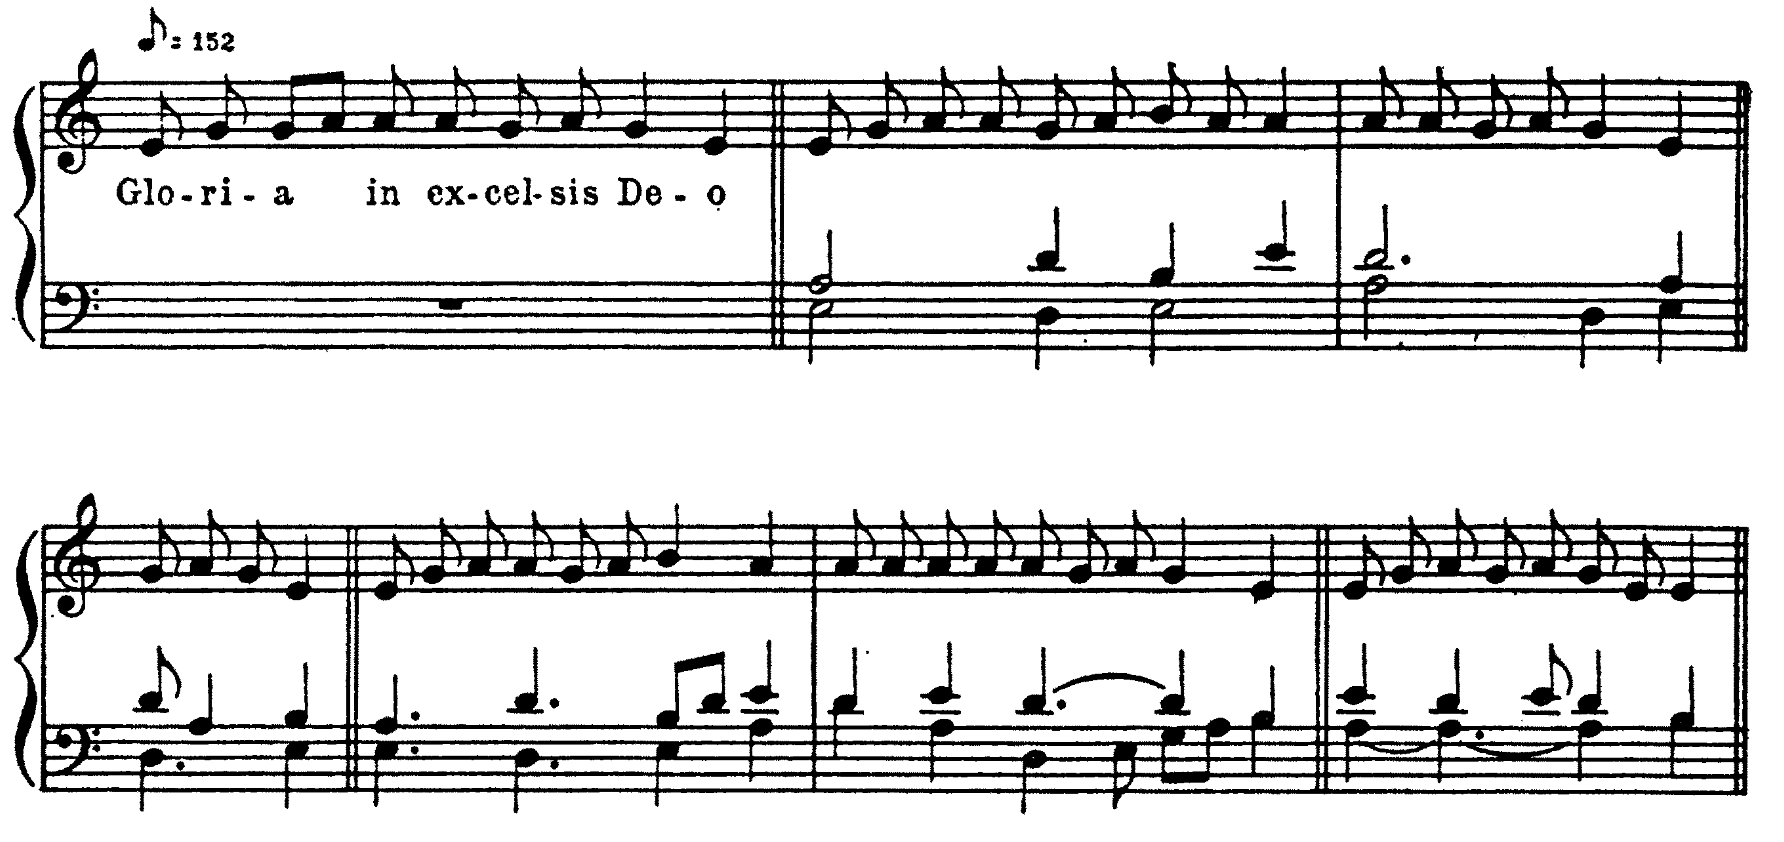
\includegraphics[width=\linewidth]{c/5/ex/yasser_quartal_360.png}
  \caption{Yasser, Quartal harmonisation, 1938}
  \label{mus:yasser_quartal_360}
\end{example}


\vspace*{\fill}

\begin{example}
  \centering
  \includegraphics[width=\linewidth]{c/5/ex/burgstahler_quartal_66.png}
  \caption{Burgstahler, \emph{Ibid}., 1957}
  \label{mus:burgstahler_quartal_66}
\end{example}


\vspace*{\fill}

\newpage

\vspace*{\fill}

\begin{example}
  \centering
  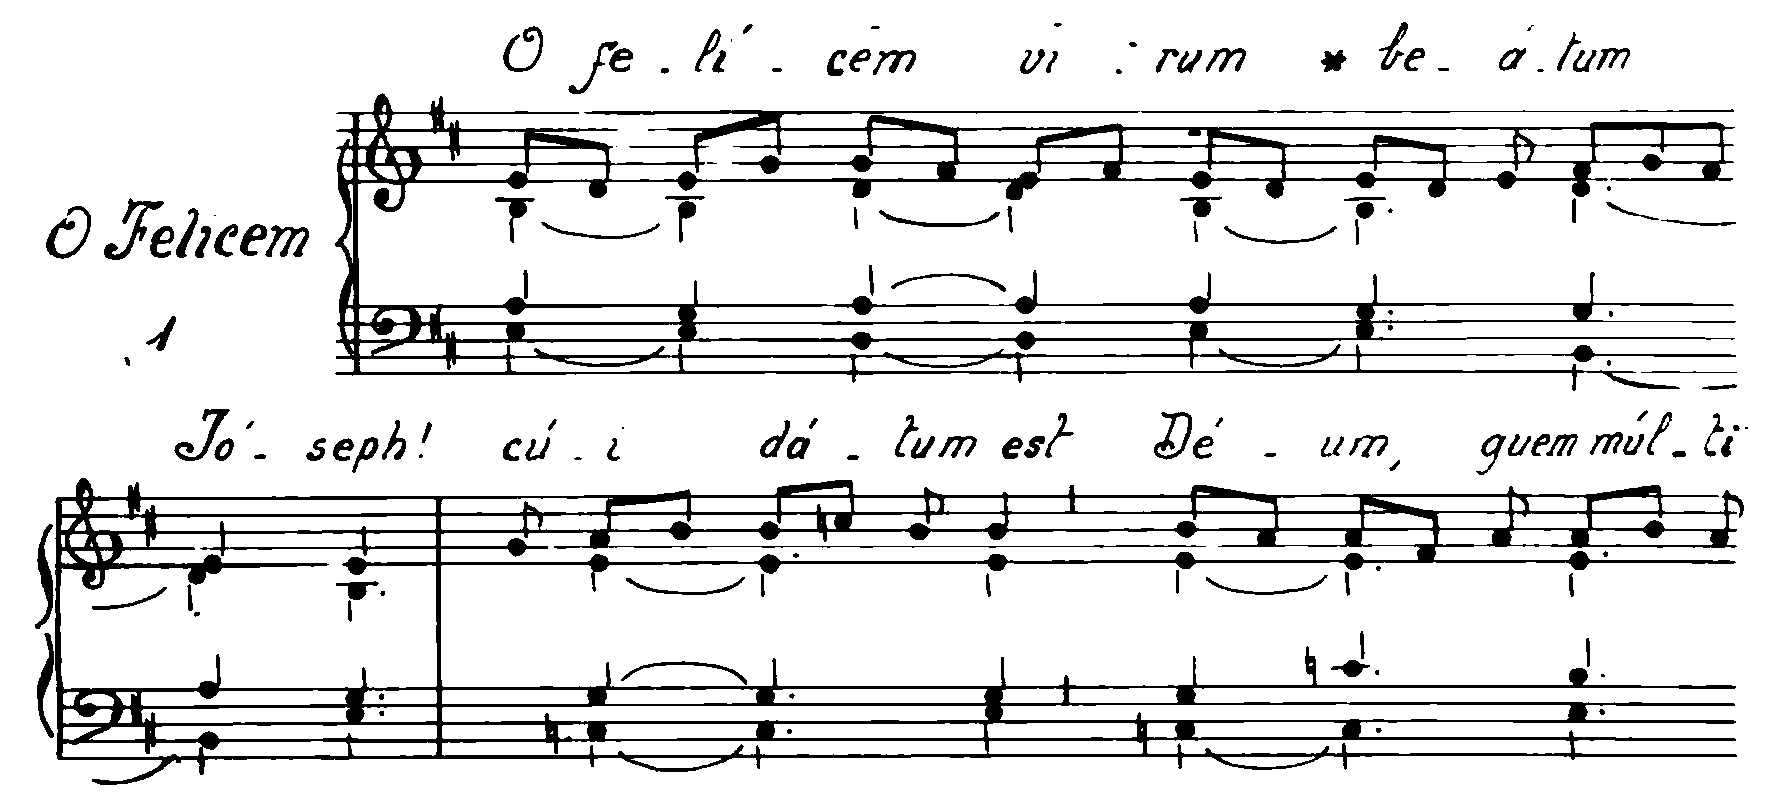
\includegraphics[width=\linewidth]{c/5/ex/gagnon_dissonant_49.png}
  \caption{Placide Gagnon, `Double rhythm', 1944}
  \label{mus:gagnon_dissonant_49}
\end{example}

\vspace*{\fill}

\begin{example}
  \centering
  \includegraphics[width=\linewidth]{c/4/ex/noh_42.png}
  \caption{\emph{Nova organi harmonia} notational style, \emph{c}.1942}
  \label{mus:noh_42}
\end{example}

\vspace*{\fill}

\newpage

\vspace*{\fill}

\begin{example}
  \centering
  \includegraphics[width=\linewidth]{c/5/ex/jones_ictus_15.png}
  \caption{Jones, Use of `C'\kern 1pt\sharp{} and presence of vertical \emph{episemata}, 1952}
  \label{mus:jones_ictus_15}
\end{example}

\vspace*{\fill}

\begin{example}
  \centering
  \includegraphics[width=\linewidth]{c/5/ex/cauter_simple_10.jpg}
  \caption{Van de Cauter, Simple style, \emph{c}.1944}
  \label{mus:cauter_simple_10}
\end{example}

\vspace*{\fill}
